\documentclass[a4,12pt]{article}
	\usepackage[UTF8]{ctex}
	\usepackage{datetime2}% to use \DTMnow
	\usepackage{indentfirst}
		\setlength{\parskip}{5pt}% spacing between paragraphs
		\setlength{\parindent}{20pt}% indentation
	\usepackage{geometry}
		\geometry{tmargin=8mm,bmargin=15mm,lmargin=8mm,rmargin=8mm}
	\usepackage{enumitem}
	\usepackage{amsmath}
	\usepackage{amssymb}% use mathcal, etc.
	\usepackage{mathtools}
	\usepackage{physics}
	\usepackage{tabu}
	\usepackage{tikz}
		\usetikzlibrary{arrows.meta,calc,decorations.markings,math,arrows.meta,patterns,angles,quotes,decorations.pathreplacing}

% self-defined commands always begin with UPPERCASE LETTER
	\newenvironment{LatinModern}{\fontfamily{lmr}\selectfont}{\par}% Latin Modern
	\DeclareTextFontCommand{\textmyfont}{\LatinModern}
	\newcommand{\Curs}[1]{\emph{\LatinModern{#1}}}
	\newcounter{Problem}
	\newcommand{\Problem}[1]{
		\vspace*{10pt}
		\stepcounter{Problem}
		\label{Problem \arabic{Problem}}
		\noindent\arabic{Problem}.\emph{~#1}
	}
	\newcommand{\Qed}{\hfill\ensuremath{\square}}

% useful symbols
	\def\Tick{\ding{51}}
	\newcommand{\rectangle}{{
		\ooalign{$\sqsubset\mkern3mu$\cr$\mkern3mu\sqsupset$\cr}
	}}

\begin{document}

% Title
	\title{
		\vspace*{-50pt}
		\Large{\textbf{太平华联中学数学竞赛题解}\vspace*{-10pt}}\\
	}
	\author{作者:郑其恩 Fanurs\vspace*{-30pt}}
	\date{最后编译时间:\DTMnow (美东)}
	\maketitle
	\vspace*{-25pt}

\setcounter{Problem}{0}
\Problem{
	下图中,$ABCDE$是正五边形。若$\angle CAD = x^\circ$,求$x$。
	\begin{center}
	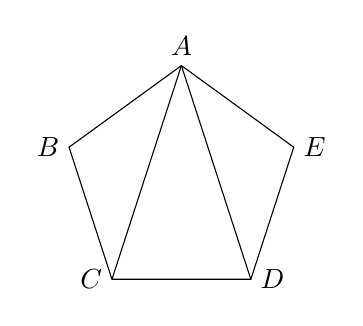
\begin{tikzpicture}[scale=1.5]
		\coordinate (A) at ({cos(90+0*72)}, {sin(90+0*72)});
		\coordinate (B) at ({cos(90+1*72)}, {sin(90+1*72)});
		\coordinate (C) at ({cos(90+2*72)}, {sin(90+2*72)});
		\coordinate (D) at ({cos(90+3*72)}, {sin(90+3*72)});
		\coordinate (E) at ({cos(90+4*72)}, {sin(90+4*72)});
		\draw (A) node[above] {$A$}
			--(B) node[left] {$B$}
			--(C) node[left] {$C$}
			--(D) node[right] {$D$}
			--(E) node[right] {$E$} --(A);
		\draw (A)--(C);
		\draw (A)--(D);
	\end{tikzpicture}
	\end{center}
	}

	五边形内角和为$540^\circ$。如果不知道的同学,可观察五边形$ABCDE$可切割为三个三角形,$\triangle{ABC}$、$\triangle{ACD}$及$\triangle{ADE}$。由于每个三角形内角和为$180^\circ$,因此五边形的内角和为$3\times180^\circ = 540^\circ$。

	由于正五边形内角和为$540^\circ$,所以每个内角皆等于$540^\circ\divisionsymbol5=108^\circ$。

	接下来我们计算$\angle BAC$。由内角和$180^\circ$,可得
	\[ \begin{aligned}
			\angle BAC + \angle ACB + \angle ABC &= 180^\circ \\
			\angle BAC + \angle ACB + 108^\circ &= 180^\circ \\
			\angle BAC + \angle ACB &= 72^\circ \ \mbox{。}
		\end{aligned}
	\]
	记得$ABCDE$是正五边形,意味着所有边长相等,包括$AB=BC$,即$\triangle{ABC}$为等腰三角形。因此$\angle BAC = \angle ACB$。由此,我们得到
	\[ \begin{aligned}
			2\angle BAC &= 72^\circ \\
			\angle BAC &= 36^\circ \ \mbox{。}
		\end{aligned}
	\]
	同理,$\angle BAC$的镜面,$\angle EAD$也会等于$36^\circ$。因此
	\[ \begin{aligned}
			\angle BAC + \angle EAD + \angle CAD &= \angle BAE \\
			(36^\circ + 36^\circ) + \angle CAD &= 108^\circ \\
			\angle CAD &= 36^\circ \\
			\therefore x &= 36 \ \mbox{。}
		\end{aligned}
	\]
	\Qed
	\vspace*{30pt}

	\noindent 点评:
	\begin{enumerate}[label=(\alph*)]
		\item 五边形的几何性质很多都可以从三角形推导而出,这就是为什么它常出现在竞赛题目,就是为了考验学生把课堂所学(通常是三角形和四边形)推广到五边形的能力。其中$AC$和$AD$是解五边形常用的辅助线,但本题因要求得$x$所以直接给出了。
	\end{enumerate}

\pagebreak
\Problem{
	求满足不等式$4\le999-3x<1000$的最大整数。
	}

	首先,我们把不等式化简。请注意当乘以负数时,不等式会倒过来。
	\[ \begin{aligned}
			4 \le 999 - 3x < 1000 \\
			4-999 \le -3x < 1000 - 999 \\
			-995 \le -3x < 1 \\
			(-1)\times(-995) \ge (-1)\times(-3x) > (-1)(1) \\
			995 \ge 3x > -1 \\
			331\frac{2}{3} \ge x > -\frac{1}{3} \ \mbox{。}
		\end{aligned}
	\]
	显然,$x = 331$是最大且又能满足不等式的整数。
	\Qed
	\vspace*{30pt}

	\noindent 点评:
	\begin{enumerate}[label=(\alph*)]
		\item 本解答采用了较为冗长但系统性的解法,学生最常犯的错就是在乘以负数时忘了把不等式倒过来。想想看,$1 < 2$,可是$-1 > -2$,对吧?
		\item 但是这题的不等式其实特别简单,数感强的同学可以很快发现“右边的条件”$999-3x<1000$并不是限制因素,因为从$999$扣掉任何正数$3x$都会小于$1000$。关键在于“左边的条件”,究竟这$999$能扣多少,而不至于少于$4$。
		\item 这两种方法,“正规法”和“观察法”都应该多练习。
	\end{enumerate}

\pagebreak
\Problem{
	求
	\[ \frac{3\sqrt{3}+5}{3\sqrt{3}-5} + \frac{3\sqrt{3}-5}{3\sqrt{3}+5} \]
	的值。
	}

	这类题目其实就是直截了当地化简。竞赛中为了加快速度,可以先设$a:=3\sqrt{3}$和$b:=5$。如此以来,式子也会看得更整齐,最后需要计算时再代入数值:
	\[ \begin{aligned}
			\mbox{原式}
			&= \frac{a+b}{a-b} + \frac{a-b}{a+b} \\
			&= \frac{(a+b)^2 + (a-b)^2}{(a-b)(a+b)} \\
			&= \frac{2(a^2+b^2)}{a^2-b^2} \\
			&= 2\cdot\frac{(3\sqrt{3})^2 + 5^2}{(3\sqrt{3})^2 - 5^2} \\
			&= 2\cdot\frac{27 + 25}{27 -25} \\
			&= 52 \ \mbox{。}
		\end{aligned}
	\]
	\Qed
	\vspace*{30pt}

	\noindent 点评:
	\begin{enumerate}[label=(\alph*)]
		\item 完全平方公式$(a\pm b)^2=a^2+b^2\pm 2ab$大家应该都会。而两个完全平方式的加减不妨也熟悉下:
			\[ \begin{aligned}
					(a+b)^2 + (a-b)^2 &= 2(a^2 + b^2) \\
					(a+b)^2 - (a-b)^2 &= 4ab \\
				\end{aligned}
			\]
			当然这些关系式真的不用硬记,一般多遇到几次就能记得了。这里特别提一下,只是为了竞赛是可以跳点步骤,加快解题速度。
	\end{enumerate}

\pagebreak
\Problem{
	若三位数$\overline{2a7}$可以被$11$整除,求$a$的值。
	}

	这里重新温故$11$的整除规则:一个数如果起“偶位数之和”和“奇位数之和”之差为$11$的倍数,则该数可被$11$整除。比如$63525$的“偶位数之和”是$2+3=5$,“奇位数之和”是$6+5+5=16$。两和之差为$11$,因此$63535$是$11$的倍数。

	若三位数$\overline{2a7}$可以被$11$整除,则根据$11$的整除法,
	\[ \abs{(2+7) - a} = \abs{9 - a} \]
	必须是$11$的倍数。由于$a$只能是介于$0$到$9$的个位数,所以唯一满足的解为$a=9$。
	\Qed
	\vspace*{30pt}

	\noindent 点评:
	\begin{enumerate}[label=(\alph*)]
		\item 请复习数的整除规则。
	\end{enumerate}

\pagebreak
\Problem{
	下课时,$1001$位学生去食堂,每位男生吃了两碗饭,每位女生吃了一碗饭,结果这些学生一共吃了$1654$碗饭。问女生有几人?
	}

	设有$x$位男生,$y$位女生。则我们可列出以下二元一次联立方程:
	\[ \begin{dcases}
			x + y = 1001 \\
			2x + y = 1654
		\end{dcases}
		\ \mbox{。}
	\]
	把第二个方程减掉第一个方程,得
	\[ x = 653 \ \mbox{。} \]
	因此,
	\[ y = 1001 - x = 1001 - 653 = 348 \ \mbox{。} \]
	\Qed
	\vspace*{30pt}

	\noindent 点评:
	\begin{enumerate}[label=(\alph*)]
		\item 这是基本的课堂题目。
	\end{enumerate}

\pagebreak
\Problem{
	有一群学生,其中$\frac{1}{3}$是男生,女生中,有$\frac{3}{8}$戴眼镜。若没有戴眼镜的女生有$45$人,问这群学生有多少人?
	}

	\begin{itemize}
		\item 女生中,有$\frac{3}{8}$戴眼镜,所以有$\frac{5}{8}$没戴眼镜。
		\item 没有戴眼镜的女生有$45$人并占了$\frac{5}{8}$,所以一共有$45\times\frac{5}{8} = 72$位女生。
		\item 这群学生中,$\frac{1}{3}$是男生,因此女生占了$\frac{2}{3}$。
		\item 所以一共有$72\times\frac{3}{2} = 108$位学生。
	\end{itemize}
	\Qed
	\vspace*{30pt}

	\noindent 点评:
	\begin{enumerate}[label=(\alph*)]
		\item 别粗心。
	\end{enumerate}

\pagebreak
\Problem{
	架子上有$23$盒蓝色原子笔及$17$盒红色原子笔。每个盒子都密封着,盒子的表面积完全一样,没有注明里面所含原子笔的颜色。林老师赶着去上课,却需要一盒红色原子笔。因此她打算先拿走若干盒原子笔,去到班上才打开找一盒红色的。林老师必须取走最少多少盒原子笔,才能保证至少有一盒是红色的?
	}

	如果是最“幸运”的情况,那林老师只要随便拿一盒就是红色的了。	但题目要我们考虑任何情况,并且是要保证带走的盒子里有红色原子笔。为此,我们假设最“倒霉”的情况,也就是林老师先是把所有$23$盒蓝色原子笔都带走了,然后再多拿一盒,则那一盒必然是红色。因此林老师必须至少取走$24$盒原子笔才能每次都保证有带上红色原子笔。
	\Qed
	\vspace*{30pt}

	\noindent 点评:
	\begin{enumerate}[label=(\alph*)]
		\item 把问题考虑成最“幸运”和最“倒霉”的情况就比较好理解了。
	\end{enumerate}

\pagebreak
\Problem{
	如下图所示,$ABCD$是一四边形,其对角线$AC$与$BD$互相垂直。若$AC=19$,$BD=22$,求四边形$ABCD$的面积。
	\begin{center}
	\begin{tikzpicture}[scale=0.8]
		\coordinate (A) at (0,0);
		\coordinate (B) at (1,-1);
		\coordinate (C) at (5,1);
		\coordinate (D) at (0,4);
		\draw (A) node[left] {$A$}--(B) node[below] {$B$};
		\draw (A) --(C) node[right] {$C$};
		\draw (A) --(D) node[above] {$D$};
		\draw (B) --(C);
		\draw (B) --(D);
		\draw (C) --(D);
	\end{tikzpicture}
	\end{center}
	}

	如果$AC$与$BD$互相垂直,那我们便能利用“补形法”,建构出以下长方形$PQRS$:
	\begin{center}
	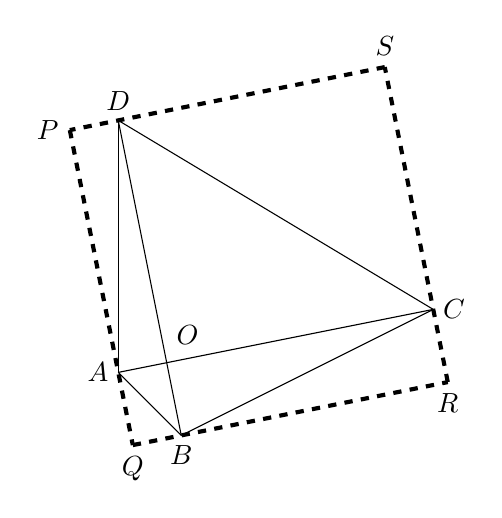
\begin{tikzpicture}[scale=0.8]
		\coordinate (A) at (0,0);
		\coordinate (B) at (1,-1);
		\coordinate (C) at (5,1);
		\coordinate (D) at (0,4);
		\coordinate (O) at ({10/13}, {2/13});
		\coordinate (P) at ({-10/13}, {50/13});
		\coordinate (Q) at ({3/13}, {-15/13});
		\coordinate (R) at ({68/13}, {-2/13});
		\coordinate (S) at ({55/13}, {63/13});
		\draw (A) node[left] {$A$}--(B) node[below] {$B$};
		\draw (A) --(C) node[right] {$C$};
		\draw (A) --(D) node[above] {$D$};
		\draw (B) --(C);
		\draw (B) --(D);
		\draw (C) --(D);
		\draw (O) node[right, yshift=10pt] {$O$};
		\draw[dashed, line width=1.5pt] (P) node[left] {$P$}--(Q) node[below] {$Q$};
		\draw[dashed, line width=1.5pt] (Q)--(R) node[below] {$R$};
		\draw[dashed, line width=1.5pt] (R)--(S) node[above] {$S$};
		\draw[dashed, line width=1.5pt] (S)--(P);
	\end{tikzpicture}
	\end{center}

	整个图形可被$AC$和$BD$切割成四份。我们以长方形$AOPD$为例,因$\triangle{AOD}$为直角三角形,所以其面积恰好为长方形$AOPD$的一半。同样的推理也适用于长方形$CODS$、长方形$COBR$及长方形$AOBQ$。因此,四边形$ABCD$的面积为
	\[ \begin{aligned}
			S(\rectangle ABCD)
			&= \frac{1}{2}S(\rectangle PQRS) \\
			&= \frac{1}{2}(\overline{AC}\cdot\overline{BD}) \\
			&= \frac{1}{2}(19\times22) \\
			&= 209 \ \mbox{。}
		\end{aligned}
	\]
	\Qed
	\vspace*{30pt}

	\noindent 点评:
	\begin{enumerate}[label=(\alph*)]
		\item 初中竞赛中最常用到的“补形法”就是把三角形补成长方形。
	\end{enumerate}

\pagebreak
\Problem{
	将$4$支一样的蓝笔与$3$支一样的红笔排成一行,其中$3$支红笔必须相邻,有几种排法?
	}

	由于题目要求$3$支红笔必须相邻,所以我们不妨把它们视为一体。由此,可列出以下排列法:
	\begin{enumerate}
		\item {\color{red}{红} \color{blue}{蓝} \color{blue}{蓝} \color{blue}{蓝} \color{blue}{蓝}}
		\item {\color{blue}{蓝} \color{red}{红} \color{blue}{蓝} \color{blue}{蓝} \color{blue}{蓝}}
		\item {\color{blue}{蓝} \color{blue}{蓝} \color{red}{红} \color{blue}{蓝} \color{blue}{蓝}}
		\item {\color{blue}{蓝} \color{blue}{蓝} \color{blue}{蓝} \color{red}{红} \color{blue}{蓝}}
		\item {\color{blue}{蓝} \color{blue}{蓝} \color{blue}{蓝} \color{blue}{蓝} \color{red}{红}}
	\end{enumerate}
	排法一共$5$种。
	\Qed
	\vspace*{30pt}

	\noindent 点评:
	\begin{enumerate}[label=(\alph*)]
		\item 在高中,这类题目一般要求学生利用“组合排列”去计算。但是对于初中生来说,面对不太复杂的题目,更好且直观的方法应该是穷举法,并且通过练习和经验的累积,确保自己能系统性地把所有可能一次列出。穷举法能培养学生对组合排列的“感觉”,对将来学习“组合排列”也很有帮助。
	\end{enumerate}

\pagebreak
\Problem{
	考完试后,老师计算班上学生的平均分数,得平均分为$70$分。后来发现少算了一位考$87$分的学生李大卫的成绩。重新计算及确认后得全班的平均分数是$71$分。问这班上(包括李大卫)有多少位学生?
	}

	假设班上,包括李大卫,一共有$n$个学生,则从题目,我们可得
	\[ \begin{dcases}
			\frac{S_{n-1}}{n-1} = 70 \\
			\frac{S_{n-1} + 87}{n} = 71
		\end{dcases} \ \mbox{,}
	\]
	其中$S_{n-1}$全班同学,除了李大卫,的分数之和。

	上述联立方程,可整理成
	\[ \begin{dcases}
			S_{n-1} = 70n - 70 \\
			S_{n-1} + 87 = 71n
		\end{dcases} \ \mbox{。}
	\]
	将第二个方程减去第一个方程,得
	\[ \begin{aligned}
			87 &= (71-70)n + 70 \\
			\therefore n &= 17 \ \mbox{。}
		\end{aligned}
	\]
	班上,包括李大卫,一共有$17$位学生。
	\Qed
	\vspace*{30pt}

	\noindent 点评:
	\begin{enumerate}[label=(\alph*)]
		\item 二元一次联立方程的基本题。参赛同学须意识到“其他学生的分数”应该以总和作为$n$以外的第二个未知数,其他同学个别的分数,由本题条件不得而知。
	\end{enumerate}

\end{document}
